\cleartoleftpage
%\begin{center}
%\vspace{2cm}
%\begin{minipage}{5in}
%\cleartoleftpage
\tikz[remember picture,overlay]
\node[opacity=0.8,inner sep=0pt] at (current page.center){
\includegraphics[width=\paperwidth,height=\paperheight]{frontmatter/images/border-1.png}};
\thispagestyle{empty} %remove page number?
\begin{center}
\vspace*{-0.5cm}
{\Large Scaling the Researcher \normalsize
\small

\vspace*{0.3cm}

\includegraphics[scale=0.1]{chapters/images/discussion/dana.png}
% image from: https://www.kissclipart.com/data-analyst-png-clipart-data-science-data-analysi-fk1hr4/download-clipart.html
\vspace*{0.3cm}

Meet Dana.
Dana is a biologist who studies DNA\@.
Dana sends her samples out to be sequenced, and gets back hard drives full of files.
However, she doesn't really know what to do with these files.
She tries opening a VCF file in Excel, but it complains that there are too many lines and immediately closes.
She double clicks on a FASTQ file, and her computer freezes while trying to open the file in Notepad.

Luckily her group has a bioinformatician, Bindi, surely they can just do the analysis for her!
Bindi tells her she is very busy right now doing analysis for the group, and can look at her files in a few months, hopefully.
Dana just wants to analyse her data and publish her paper! She doesn't want to wait months, so she tries analyzing her data herself.
She finds some tools in the literature but when she tries to install them, she sees they cannot be run on Windows, what now?
She gets access to a Linux compute server, but the tool she wants does not install properly.
There are no good instructions on how to fix the problem.
She tries a different tool, which does install, but when she runs it on her own data, she gets some cryptic error messages.
\emph{``Only bioinformaticians could make sense of all this!''}, she sighs.

Then somebody tells her about Galaxy.
It has the tools she wants, and she doesn't even have to install anything, all she has to do is click buttons in her browser!
And it's free!
Galaxy is not easy, but there are a lot of useful training materials available.
She teaches herself how to use Galaxy, and how to analyze her data. She reads papers and reproduces their methods in Galaxy.
She gets stuck, but asks for help from the community.
She goes to workshops to learn more.
It was a lot of work, but she gets some promising results! She has another batch of samples on the way. She creates a workflow to speed up the analysis next time.

Her coworkers also want to analyze their data.
Bindi the bioinformatician is still very busy, and the queue is long, so they ask Dana for help.
Dana shares her Galaxy workflow with them.
She gets a lot of emails with questions from her coworkers, so she decides to create her own Galaxy tutorial about the workflow.
Dana teaches a workhops, training her colleagues on how to use Galaxy and her workflow.

Dana publishes her paper. Dana is happy.
With researchers in the group now running their own day-to-day analyses, Bindi the bioinformaticians has more time.
She can use this time to add new tools to Galaxy, create workflows for the group, and develop training materials for her coworkers to use. Bindi is happy too.
\normalsize
}
\end{center}
%\end{minipage}
%\end{center}

\cleartorightpage

\begin{savequote}[75mm]
``Humans are allergic to change. They love to say, `We've always done it this way.'' I try to fight that. That's why I have a clock on my wall that runs counter-clockwise.''
\qauthor{Grace Hopper}
\end{savequote}

\chapter{Discussion}\label{discussion}
\setcounter{figure}{-1}
\setcounter{table}{-1}
\setcounter{section}{-1}
\setcounter{NAT@ctr}{-1}

\begin{figure}[t!]
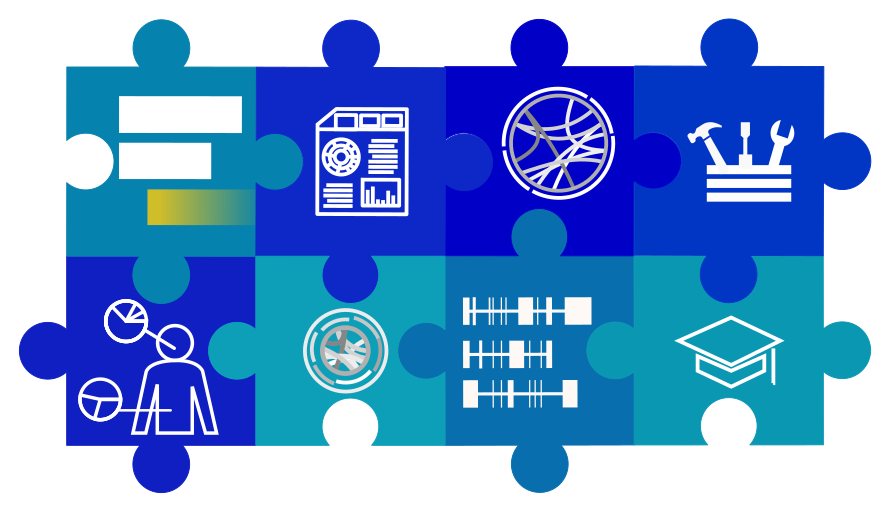
\includegraphics[height=15em]{frontmatter/images/chapter-header-discussion-tools.png}
\end{figure}
\setcounter{figure}{-1}
\setcounter{table}{-1}
\setcounter{section}{-1}


\emph{``Bioinformatics has become too central to biology to be left to specialist bioinformaticians''} notes Lincoln Stein in 2008 \cite{stein2008bioinformatics}.
And indeed, bioinformatics now plays a vital role in almost every biological and biomedical research project.
Data is being generated at an exponential rate, but bioinformaticians are not,  and it is not scalable to leave the analysis of all this data to specialist bioinformaticians.
Much of the discussion around the challenge of scaling to meet the needs of this data deluge tends to focus on the need for scaling up compute resources and data storage.
And while these are both very important factors, the much greater challenge lies in scaling not just the analysis itself, but the interpretation of all this data.
And nobody is better suited for this task than the research scientists themselves. So the question now becomes: \emph{How can we scale the researcher?}

The answer to this question lies in empowering researchers to run their own data analyses again.
The way we achieve this is by shining a light in the black box of bioinformatics.
This entails making bioinformatics tools and pipelines accessible and easy to use for domain scientists.
It requires training of researchers not just in how to use these tools, but also basic knowledge about the computational methodologies, and any biases these may introduce that can impact the interpretation of results.

This is not to say there is no role for bioinformaticians.
It takes a lot of work to make analysis accessible, but by enabling research scientists to handle their own day-to-day analyses, we free up bioinformaticians to focus on the development of new and better tools, configuring new workflows, improving reproducibility, and developing and delivering training.

Therefore, in this thesis we set out to develop a user-friendly, open, and FAIR bioinformatics framework for NGS analysis, so that we can create a community of researchers who are computationally informed.
We then applied this paradigm to a series of research projects to illustrate its utility.


%Since the completion of the human reference genome in 2003, the field of molecular biology has been transformed almost beyond recognition, and along with it, the field of bioinformatics has evolved from a niche discipline to an integral part of every biomolecular research question. Where decades ago most genomic data analyses could largely be performed by hand, nowadays they often require a supercomputer. Programming knowledge is required to run such analyses, but biomedical scientists are not typically trained in these skills, and have thus become reliant on bio\-infor\-ma\-ticians to carry out this work for them. Similarly, bioinformaticians often lack the increasingly complex biological knowledge required to fully interpret the results~\cite{preeyanon2014reproducible}. Biologist and bioinformatician must therefore work together closely, and each should be trained in the other discipline in order gain awareness of factors that might influence analysis or result interpretation.

%Furthermore, data is being generated at an exponential rate (while bioinformaticians are not), and one way to address this gap is to empower researchers and clinicians to run their own day-to-day analyses without the need to consult a bioinformatician at every step. A way towards delivering this is through the creation of accessible analysis tools and platforms and sufficient training resources.


\section{Accessible Bioinformatics}

The main challenge in our aim of scaling the researcher, is making bioinformatics accessible for non-bioinformaticians. This includes not only making analyses easy to use, but also easier to understand and interpret.
In our approach we used the Galaxy platform to provide a user-friendly interface to bioinformatics analyses. Galaxy does all the heavy lifting of handling installation of the tools and all their dependencies, of optimally scheduling jobs across the compute resources, tracking provenance of analyses, enabling sharing, and much more. This leaves the researcher free to focus on the interpretation of their results.
The second main component of our approach to making bioinformatics more accessible consists of providing extensive bioinformatics training. To this end, we founded the Galaxy training materials project, a collaborative framework for development and maintenance of training materials using the Galaxy framework.


\subsection{Galaxy as a user-friendly workflow platform}

The Galaxy project~\cite{giardine2005galaxy,blankenberg2010galaxy,afgan2016galaxy} enables researchers to run complex data analysis without programming expertise, directly from their web browser. While there are several workflow management systems \cite{clcbio,taverna,onlinehpc,anduril,molgenis}, some of these solutions are commercial and may not be affordable to many labs, and others require local installation, prohibiting scaling to accomodate large datasets. Furthermore, many solutions are not open source, meaning only the core development team can provide updates to the platform, limiting flexibility of the platform to its end users.

In contrast, Galaxy is completely free and open-source, and perhaps its most attractive asset is the very large and active user and developer community behind it. Galaxy encourages feedback and code contributions from its users to improve the platform, and evolve along with the ever-changing landscape that is bioinformatics. This paradigm means that anybody is able to add features to Galaxy or provide bug fixes, and can share those enhancements back to the main code base, thereby enabling a much faster and more flexible development cycle.

Galaxy continues to increase in popularity, illustrated by the exponential growth of both the number of available tools (over 8000) \cite{galaxytoolshed}, and the number of publication citing Galaxy (almost 10,000) \cite{url-zotero-galaxy}.
\hyperref[chapter:galaxy]{\textbf{Chapter~\ref{chapter:galaxy}}} outlines the ongoing development in the Galaxy framework. One of the major improvements was in the handling of big data. Galaxy addresses this issue by introducing the concept of data collections. This allows users to easily scale their analyses up from single datasets to hundreds of thousands of samples at once, using the exact same procedures they have grown accustomed to.
However, the greater challenge of big datasets is not just the processing of the files, but rather managing all this data in an effective way.
To support the organisation of these large number of samples in Galaxy, the rule-based uploader was created, a novel feature which essentially allows sample sheets to be uploaded alongside the raw data files, and the metadata stored within them to be coupled to the datasets in Galaxy.

While the Galaxy project certainly greatly improves accessibility of bioinformatics analyses, there are still a number of areas of improvement remaining.
For example, with sequencing now widespread and affordable, it has become feasible to use NGS directly in the clinic to inform patient care.
However, until now Galaxy has focused mainly on researchers, and in order to make Galaxy more appealing for clinicians, the framework could benefit from a number of additional features.
Firstly, a \emph{locked-down}, workflow-centric user interface is required; in contrast with research applications where Galaxy's great flexibility is an asset, for clinical applications this flexibility can be a hindrance, as it goes hand in hand with added complexity.
Unlike researchers, clinicians do not typically need to play around with their datasets and try different tools; their analysis options should be limited to a small set of predefined and thoroughly validated analysis pipelines.
While Galaxy does not (yet) offer such an alternate user view, it does offer API access to its framework, enabling custom front-ends to be developed on top of the Galaxy back-end.
The need for such a simplified user interface to Galaxy is exemplified by the number of projects that have developed such a customized front-end to the Galaxy interface \cite{klingstrom2017galaksio,matthews2018integrated,lemoine2019ngphylogeny,SEEK2015}, including several in-house projects at the ErasmusMC\@.
For example, the IRIDA (Integrated Rapid Infectious Disease Analysis) project \cite{matthews2018integrated} is an open-source platform for public health genomics, which is currently in use by the Canadian public health department to track infectious disease outbreaks.
It uses Galaxy as its analysis platform, but provides a custom user interface tailored specifically to the needs of its users. This approach also enabled the project to integrate Galaxy directly with a third-party data management system where users can easily mange their projects and data.
While Galaxy does not aim to be a data management system, in this big data era it has become increasingly imperative to offer good data management solutions to researchers. Therefore, integrations of Galaxy with third-party data management systems in the future could profoundly increase usability of the platform even further.

We used Galaxy as the main data analysis platform in each of the 3 research projects described in this thesis, including one clinical analysis platform (MYcrobiota). For several of these publications, we were able to submit our Galaxy history and workflows directly to the journal as a full end-to-end demonstration of our analysis pipeline, which could then be used to reproduce our results by reviewers and readers.


\subsection{Visualisation and Reporting}
Visualisation is an essential component to aid in interpretation of big and multidimensional datasets. Tools such as Circos \cite{circos} allow for the visualisation of multiple large and complex datasets in a single circular plot. Circos is highly customizable, but this high degree of flexibility comes paired with a high degree of complexity and a steep learning curve. To improve the user-friendliness of this tool and improve its interoperability with upstream tools, we developed Galactic Circos (Chapter~\ref{chapter:general}), integrating Circos into Galaxy, and providing a set of preprocessing tools to facilitate interoperability with a wide range of output formats produced by upstream tools.

The Circos visualisation tool was especially useful in discovery of chromothripsis of the VCaP sample (Chapter~\ref{chapter:vcap}).
Here the highly rearranged nature of chromosome 5q was instantly obvious in one glance at the circular plot, in a way that simply inspecting the textual files listing the SVs could not convey.

Effective visualisation of large data is crucial for the interpretation of analysis results, and in a broader sense, so is the reporting of results in a single, easily-digestible overview or report. Analysis pipelines often result in a large set of different output files, and displaying these results effectively to the end user tasked with interpretation of the results is a challenge in its own right.
Galaxy in its current form lacks an appealing system of results summation and reporting. While Galaxy sports a plugin system for visualisation of individual datasets, a generic reporting tool for displaying a set of workflow outputs together does not exist. To this end, we developed iReport (Chapter~\ref{chapter:general}); a fully customizable Galaxy tool for the generation HTML reports capable of displaying any number of workflow outputs.\

iReport is intended to be used as the final step of a workflow, and is generic enough that it makes no assumptions about the underlying analysis or scientific domain.\ iReport supports  the ability to add links to datasets and external resources, create searchable and sortable tables, embed images and custom text, and to structure content into different pages.
By adding such a summarizing report at the end of an analysis pipeline, clinicians and other end users are able to run workflows and view results with minimal instruction or knowledge of the Galaxy interface.
We used iReport as the reporting tool for the MYcrobiota clinical analysis platform (Chapter~\ref{chapter:mycrobiota}), based on the requirements of the clinicians at the Streeklab Haarlem.

Since the development of the iReport tool, the need for a reporting system more tightly integrated with the Galaxy framework itself was recognized by the Galaxy core team, and they have since started to integrate similar functionality into the Galaxy code base. While this reporting system is relatively new and does not yet support the full functionality of iReport, we are hopeful that continued development here will improve Galaxy's reporting mechanisms.

\subsection{Training}
Training is an essential component in the dissemination of accessible bioinformatics tools and workflows. The Galaxy platform is especially well-suited for the delivery of bioinformatics training because it provides a layer of abstraction that allows trainees to focus on the bioinformatics \emph{concepts} rather than the implementation details of the tools. Without this separation, trainees would have to simultaneously learn about the UNIX commandline or programming environment, on top of the bioinformatics topics at hand. This would increase the cognitive load and hamper the learning process~\cite{paas2003cognitive}. Given this observation of Galaxy's suitability for use in training, the Galaxy Training Network (GTN)~\cite{url-gtn} was formed; a loosely-defined open group of instructors around the world who use Galaxy for training purposes. Initially there was little coordination between the different instructors in terms of materials used, and thus a lot of duplication of effort. There was a clear need for centralisation of training materials and knowledge sharing within the trainer community. Chapter~\ref{chapter:training} describes the community-driven web-based framework for the delivery of bioinformatics training using the Galaxy platform that we developed in response to this need.
Our aim was to create a fully open and transparent framework that is accessible and easy to use for both trainees and trainers. The materials are centered around \emph{research stories}; usually the recreation of results described in published papers. This gives trainees the confidence that the tools and pipelines are practically useful and of publication-level quality, as well as providing them with the opportunity to dive deeper into the science and informatics behind the training. Since the creation of this training platform, a number of scientific publications have included Galaxy training materials as a form of documentation and illustration of the presented analysis pipelines~\cite{gruning2017rna,blank2018disseminating,batut2017asaim,hiltemann2018galaxy}.

One of the main challenges in designing this framework was to allow easy contributions from instructors, without the need for any web development knowledge. To this end, we used Jekyll templating~\cite{url-jekyll}, which allows tutorials to be written in the simple and accessible markup language called Markdown~\cite{url-markdown} which can be rendered as HTML\@. Analogous to how Galaxy allows scientists to run analyses while being abstracted away from the implementation layer of the tools, this approach allows instructors to create web pages for their tutorials without being concerned with the syntax and intricacies of the web application layer.

A further challenge was to enable the materials to be usable both by instructors during workshops, and by individuals learning on their own. This is accomplished by including all materials instructors might provide during a workshop in the GTN training materials framework. This includes introduction slides as well as hand-on materials, input datasets and workflows, further reading suggestions, and an automatically updated list of available Galaxy servers which meet the requirements to run a given tutorial. Furthermore, learning assessments are provided in the form of question boxes, answers to which are included within the materials (in an initially hidden state) for trainees to verify their understanding of the materials. If further assistance is required, links to support channels such as a help forum and chat rooms are provided.

The community-driven nature of the training framework is essential for the long-term survival of the project; it allows for the distribution of the maintenance burden and takes advantage of the combined expertise present in the community. All development happens on GitHub~\cite{url-github}, where anybody may suggest additions or changes, and any such proposed changes are thoroughly tested using the Travis continuous integration system~\cite{travis-ci} to ensure functionality and adherence to guidelines. The proposed changes are subsequently reviewed by one or more of the dedicated topic maintainers, or other volunteers from the community. Once approved, the code is merged into the main code base, and the new website is automatically built and deployed using Travis and GitHub. In order to assess the quality of the tutorials and identify areas of improvement, feedback from both trainees and instructors is indispensable. To this end, we integrated evaluation forms at the end of each tutorial, and hold regular community meetings with training developers and trainers.

As Galaxy evolves, so will the associated tutorials; where Galaxy is expanding beyond bioinformatics and is now also being used in fields such as natural language processing and computational chemistry, so have we noticed a steady expansion of topics and tutorials contributed by the community. In the year following the publication of Chapter~\ref{chapter:training} , we saw 6 new topics added, 66 new tutorials, and the number of contributors grew from 64 to 137.

While the focus of development in this project initially lay with improving the experience for end-users of the tutorials, our focus is now shifting to increasing support for tutorial contributors and instructors intending to use our materials. The main challenge in the coming years will be the community management; creating and sustaining a close-knit community of Galaxy users and instructors so that the project can survive even when its original developers have moved on.

While this project focuses on the training of research scientists to effectively use bioinformatics analyses, the reverse is also important; much like bioinformatics may feel like a \emph{black box} to researchers and clinicians, so can the wetlab seem like a black box to many bioinformaticians.
Bioinformaticians typically work on multiple projects at the same time, often covering a variety of different scientific domains, and therefore can not acquire the same level of knowledge about the underlying biology as the domain specialists.
However, similar to how researchers and clinicians will benefit from a basic knowledge of computational concepts to aid the interpretation of analysis results, so do bioinformaticians need a minimum knowledge of the scientific domains in order to optimally develop their tools and workflows.
The tutorials in the GTN framework are generally aimed at novices and as a result can also be used by bioinformaticians to acquire knowledge of the basic concept involved in different scientific domains.
However, I would love to see a project conceptually similar to the GTN training materials framework, but explicitly aimed at training bioinformaticians in the relevant biological concepts.


\section{Use Cases}

The concepts and tools described in the previous sections were applied to two separate use cases. Chapters~\ref{chapter:fusiongenes} and~\ref{chapter:virtualnormal} describe the creation of analysis tools and pipelines for variant analysis in prostate cancer research. In Chapter~\ref{chapter:microbiota}, Galaxy-based analysis pipelines were developed and tested for the application of NGS-based microbiota profiling for clinical diagnostics.


\subsection{Cancer Analysis: Structural Variant Analysis}
\subsubsection{The Bio}

Cancer is a disease of the genome, where DNA mutations accumulate over time and wreak havoc on the cell. Our best hope in defeating this disease lies in the full characterization of the cancer cell, not only in terms of their observed mutational signatures, but also the mechanisms behind these mutational landscapes.

While small-scale mutations that affect the protein-coding regions of the genome have been widely studied, the impact of non-coding mutations and large-scale structural variants (SVs) in cancer remains largely undefined~\cite{cuykendall2017non,khurana2016role}. Now that whole-genome sequencing has become more available and affordable, a comprehensive characterization of SVs has become possible.

Large-scale genomic rearrangements have the potential to lead to the generation of hybrid genes known as fusion genes.
Accurate detection of such fusion genes may aid in the diagnosis or treatment of cancer~\cite{nowell1960chromosome,nowell1961chromosome,druker2001activity,druker2001efficacy}.
Prostate cancer was among the first solid tumours demonstrated to harbour frequent large-scale genomic rearrangements, demonstrated by the discovery of the \emph{TMPRSS2-ERG} fusion gene, which was found to be present in approximately 50\% of all prostate cancers \cite{tomlins2005recurrent}.
Subsequent studies have shown that point-mutations occur relatively infrequently in prostate cancer as compared to structural variations and extensive copy-number variation, suggesting that it is these large-scale genomic rearrangements that are the primary driver of prostate cancer progression \cite{taylor2010integrative,rubin2011common}.

Understanding the mechanisms behind the acquisition of these structural variations will provide valuable insights into tumor progression.
While historically the acquisition of mutations in tumour cells has been thought of as a gradual and incremental process, subsequent insights have uncovered several mutational processes capable of generating large numbers of mutations in a single event \cite{cortes2020comprehensive,willis2015}.
Kataegis (from the greek word for thunderstorm) represents a \emph{mutation storm} of localised hypermutations, and has been observed in multiple cancer types \cite{nik2012mutational,davis2014somatic}.
Chromothripsis is a shattering of the genome -often an entire chromosome or chromosome arm-, followed by a highly erroneous repair step \cite{stephens2011massive,maher2012chromothripsis}.
Chromoplexy (from the Greek \emph{pleko}, which means to weave) is a phenomenon where large chains of rearrangements affecting multiple chromosomes occur \cite{shen2013chromoplexy}. All these mechanisms challenge the classical view of cancer progression as a gradual and step-wise process.

In Chapter~\ref{chapter:vcap} we showed that chromothripsis also occurs in prostate cancer, by describing the identification of chromothripsis in the 5q arm of the VCaP cell line. A very large number of SVs were detected, and copy number varied primarily between two copy number states, with only sporadic occurrences of a third state. This alternation between a small number of copy number states suggest the rearrangements were precipitated by a single catastrophic event.
Other studies have also observed chromothripsis in other prostate cancer samples \cite{wu2012poly,Baca2013}.

Such a high degree of genomic rearrangement has the potential of contributing to cancer progression e.g.\ through activation of oncogenes, or inactivation of tumor surpressor genes.
To investigate this further, we investigated the 573 rearrangements involving the impacted region of chromosome 5 for their potential to lead to the formation of fusion genes, using the iFUSE application presented in Chapter~\ref{chapter:ifuse}.
Out of this large number of rearrangements, a relatively small number (18) were found to occur between two different genes at a consistent orientation, with only 2 predicted to be in-frame by the iFUSE application.
Out of the 18 fusion candidates identified, 16 were confirmed on the DNA level using custom PCR\@.
Only 5 of these were also measured on the mRNA level, suggesting instability of the fusion transcripts or down-regulation of the expression of these fusion genes.
Therefore, our results suggests that chromothripsis does not preferentially impact coding regions and that there is no positive selection for in-frame fusion transcripts.

Overall, our research has shown that any studies involving this commonly used prostate cancer cell line should take the presence of chromothripsis on chromosome 5q into account.
Furthermore, this study highlights the potential utility of this cell line as a model for research on chromothripsis.

Chromothripsis has been observed in many other cancer types as well, with the frequency of occurrence varying greatly across tumour types \cite{cortes2020comprehensive,voronina2020landscape,Koltsova2019,kloosterman2014prevalence}.
A study examining 2,658 WGS patient samples across 38 cancer types generated by the ICGC and TCGA projects found prevalences of chromothripsis that ranged from 100\% for liposarcomas and 77\% of osteosarcomas on the high end, to thyroid adenocarcinomas (3.3\%) and chronic lymphocytic leukemia (1.2\%) on the lower end of the spectrum \cite{cortes2020comprehensive}.
It must be noted that due to the variability in detection methods and in the precise definition and criteria of chromothripsis used in different studies, the exact numbers vary significantly in the literature, though the variability across different tumour types is consistently observed.

Chromothripsis has been shown to be associated with poorer outcomes \cite{fontana2018chromothripsis,Hirsch2012,magrangeas2011chromothripsis,molenaar} and accurate detection of the presence of chromothripsis could therefore provide clinically relevant prognostic value.


%Prostate cancer is one of the most commonly diagnosed cancer types in men, and while many patients present with an indolent form of the disease, others develop a highly aggressive tumour type, and overall, prostate cancer is among the top 10 leading causes of cancer-related deaths in men~\cite{jemal2010global}.
%Cancer is a disease of the genome, where accumulation of mutations over time drive the progression of the illness. Genome sequencing approaches can be used to extensively explore these genomic alterations in cancer, including small variants and larger structural variants (SVs), within or ouside genes.

%The advent of whole-genome sequencing techniques has enable the characterization of SVs and other mutations not detectable by exome-based approaches.
%Fusion genes may arise when structural variants (SVs) occur within two different genes, causing the creation of hybrid genes with the potential to produce hybrid proteins that may disrupt vital cell functions.
%For example, the presence of the \emph{TMPRSS2-ERG} gene fusion is observed in approximately 50\% of prostate cancer patients and many other less frequent fusions have also been identified~\cite{tomlins2005recurrent}. Detection of fusion genes may aid in the diagnosis or treatment of cancer~\cite{nowell1960chromosome,nowell1961chromosome,druker2001activity,druker2001efficacy}.

%Chromothripsis is a phenomenon observed primarily in cancer cells, that involves the shattering and subsequent imprecise repair of one or more chromosomes in a single catastrophic event. Chromothripsis is characterized by the observation of 1) large numbers of chromosomal rearrangements on a localized parts of the genome, 2) alternations between a small number of different copy number states, and 3) alternation between regions displaying a loss of heterozygosity (LOH) and those with preserved heterozygosity~\cite{maher2012chromothripsis}.



%chromoplexy (chains) in PCa - \cite{Baca2013}


\subsubsection{The Informatics}
Whole-genome sequence experiments typically generate very large output files. Furthermore, in the case of structural variant analysis, the output file formats lack consistency across tools and sequencing platforms, and interpretation is greatly aided by visualisation and annotation with external data resources. To this end, the iFUSE application was developed, creating a visual representation of fusion gene candidates and computing various metrics such as predictions of fusion protein product.

While iFUSE provides valuable aid in interpretation on a per-event basis through its visualisation and annotation, it is less suitable for obtaining a genome-wide overview of structural rearrangements. Large-scale rearrangements such as chromothripsis for instance are easy to miss when examining the raw textual output files or the iFUSE visualisations. In order to evaluate the presence of chromothripsis, a more high-level view of the genome is needed, and to that end, whole-genome visualisations were created using Circos~\cite{circos} for rearrangements, and GNUplot~\cite{url-gnuplot} for the copy number and heterozygosity plots. This approach enabled the instant identification of chromothripsis present in the VCaP sample, which could then be followed up by closer examination of individual rearrangements involving the chromosome 5q using iFUSE.

Both the iFUSE application, the Circos Galaxy wrappers, and the other tools and visualisations created in this chapter are open-source and publicly available on an example server, and are accompanied by extensive documentation to enable re-use by institutes that may have legal restrictions about the use of clinical samples on public servers.

If we want to go beyond the mere detection of chromothripsis to the prediction of the effects of these catastrophic events on the cell, we will have to fully reconstruct the tumour genome.
While algorithms have been developed for the reconstruction of structurally rearranged genomes \cite{prego,Baca2013}, none of these methods is currently capable of handling the high degree of rearrangement observed in some cancers, let alone those harbouring chromothripsis.
This appears to be a limitation of the power of the data yielded by short-read techniques, rather than a shortcoming of the algorithmic methods.
The recent advances in long-read sequencing techniques will provide valuable improvements for reconstructing cancer genomes impacted by chromothripsis by providing reads spanning multiple breakpoints.
Indeed, a recent paper described the successful reconstruction of a genome displaying chromothripsis in a patient with the rare genetic Langer–Giedion syndrome~\cite{lei2020long}.
Similar approaches could be used to reconstruct tumour genomes and have the potential to significantly increase biological insight into the effects of chromothripsis events on the cell.

\subsection{Cancer Analysis: Somatic Mutation Determination}
\subsubsection{The Bio}
One of the main challenges in analysis of oncological samples is the identification of those mutations that potentially function as oncogenic drivers, and the large number of passenger mutations or polymorphisms present in the germline of the patient that are typically deemed to be functionally benign~\cite{lawrence2013mutational}. To this end, a sample of normal tissue from the same individual is often sequenced in conjunction with the tumour sample. This allows the subtraction of germline variants from the set of mutations detected in the cancer sample, in order to narrow down the set of potential driver mutations. However, in practice such an associated normal sample may not always be available, for a variety of reasons. In such cases, an alternative approach is required.

Given the observation that the majority of any individuals germline variants are polymorphic and observed frequently throughout the human population~\cite{10002010map,10002012integrated}, in combination with the exponential increase in publicly available genomic datasets, we explored the feasibility of constructing a so-called \emph{virtual normal}, consisting of a reference set of variants found in the population. Chapter~\ref{chapter:virtualnormal} describes this investigation.

Our approach used a set of over 900 publicly available whole genomes from healthy, ethnically diverse individuals. We combined this with the customary approach of annotating variants for presences in several online databases of polymorphism in the human population. We tested the performance of our method using 4 different tumour samples with associated normal samples, 2 of which had been sequenced on two different platforms (Complete Genomics and Illumina).

Our results show that while highly unique personal variants cannot be 100\% corrected for, a significant number of variants observed in the tumour sample also occur in the virtual normal set of genomes, and thus can be corrected without the need of an associated normal sample from the same individual. As more and more WGS samples are made publicly available, increasingly rare variants may be corrected for in this manner. Furthermore, we demonstrated that the use of a virtual normal provided a significant improvement over relying solely on annotation with online variant databases. This observation seems counter-intuitive given that these databases often contain variants originating from tens of thousands of sequencing experiments; far more genomes than the virtual normal. However, this result can be explained by noting that the virtual normal approach preserves the genomic context of variants (e.g.\ adjacent variants in the same sample), while this contextual information is lost when variants are submitted to variant databases. To understand why this contextual information is so important, one must realize that many mutations can be described in multiple different yet equivalent ways, and the only way to resolve this equivalency is to take the genomic neighbourhood of the variants into account. This enables more advanced comparison algorithms to resolve equivalency of variants where routine position-based exact comparison method fall short.

A combination of all 3 correction methods (matched normal, virtual normal, and variant databases) yields optimal results, but when faced with a choice between a virtual normal or a matched normal, both approaches performed roughly equally well. Without an associated normal, personal germline variants may be erroneously deemed somatic, but conversely, omission of the virtual normal led to a roughly equal number of false-positive somatic variants. This can be explained by a combination of sequencing errors or suboptimal variant calls in the associated normal sample, and the general difficulty present in variant comparison analyses.

Depending on the use case, the decrease in power to detect highly personal germline variants may be offset by the decrease in cost from the absence of the necessity of sequencing a matched normal sample with every tumour sample.

\subsubsection{The Informatics}
The samples in this study were sequenced by Complete Genomics~\cite{drmanac}, a sequencing service which delivers both raw sequencing data and post-processed results. Complete Genomics provide a suite of commandline tools for handling and downstream analysis of their often custom file formats. As a first step towards building the virtual normal analysis pipelines, these existing tools were wrapped into Galaxy. On top of these third party tools, several custom analysis components had to be created, as well as several file format conversion steps to function as a \emph{glue} between steps. The full suite of analysis tools has been made publicly available on GitHub, as well as detailed instructions on where to obtain the virtual normal genome set, and how this may be extended with additional normal samples in the future.


\subsection{Microbiota Profiling for Clinical Diagnostics}
\subsubsection{The Bio}
The MYcrobiota project described in Chapter~\ref{chapter:microbiota} was aimed at developing a 16S microbiota profiling pipeline suitable for use in clinical diagnostics. The MYcrobiota platform is the result of a close collaboration with Streeklab Haarlem~\cite{url-streeklab}, a microbial diagnostics lab servicing a large number of GPs and hospitals in the region.

While 16S rRNA sequencing is a relatively well-established technique, there are several obstacles to overcome to enable its use in routine diagnostics. These obstacles include 1) the high prevalence of chimera formation during PCR amplification~\cite{huttenhower2012structure}, 2) the inability to standardize the relative abundance results obtained from 16S profiling across different studies, and 3) the lack of a user-friendly bioinformatics pipeline that can be operated by clinicians without extensive bioinformatics knowledge. The MYcrobiota platform addresses obstacles; the first obstacle is overcome by using a novel PCR method, and the latter two obstacles are overcome through the creation of a Galaxy-based FAIR analysis platform adhering to the bioinformatics best practices outlined in this thesis.

In order to facilitate the use of 16S rRNA sequencing in a diagnostic setting, several enhancements to standard procedure were required, both in the wet lab and the bioinformatics pipelines to overcome the aforementioned obstacles.
While chimera formation can be detected using in-silico methods, after which those sequences are typically removed from the dataset, it would of course be preferable to prevent their formation altogether. The MYcrobiota pipeline utilizes the micelle PCR (micPCR) method~\cite{boers2015micelle,boers2017novel}. In this approach, PCR amplifications of each template 16S template sequence occurs in a physically distinct reaction environment called a micelle, thus greatly reducing the generation of hybrid sequences known as chimeras. The in-silico methods for chimera detection are still included in the workflow, and can now serve the additional purpose of providing quality control metrics for the effectiveness of the micelle method of a given run.
Traditionally, 16S rRNA sequencing can only be used to provide relative abundance information, due to PCR competition induced bias. However, by utilizing the micelle PCR method, this bias is eliminated, allowing absolute quantification of abundance, allowing us to provide additional clinically relevant information in the MYcrobiotat platform.

When dealing with clinical pipelines, validation is crucial. This validation needs to occur at multiple levels; each of the tools needs to be verified to work as expected. The Galaxy platform provides a framework for incorporating technical validation tests into the tool definitions themselves; by utilizing Galaxy in our application, we automatically gain the benefit of these technical validation tests. In a similar fashion, Galaxy allows specification of workflow-level validation tests, allowing us to validate the interplay of the different tools in our workflow. Aside from these technical validation steps, experimental validation must be part of the analysis protocol. Therefore, within the MYcrobiota standard, each sample is sequenced in triplicate and averaged in order to eliminate any remaining quantification bias in the micPCR protocol. Furthermore, a negative control sample is included in each batch, and finally, an internal calibrator (IC) was used to enable quantification of each resulting OTU in terms of the number of gene copies rather than relative abundances. This IC consisted of a known quantity of a bacterium not present in the natural microbial flora under investigation, and was added to the samples before PCR amplification. By incorporation all these validation methods in the MYcrobiota application, we increase confidence in the results of the analyses, and allow us to more quickly identify potential problems when they arise.

The MYcrobiota approach was evaluated through the analysis of 47 clinical samples obtained from patients presenting with a variety of damaged skin conditions, and results were compared to the culture-based methods currently employed for routine clinical microbial diagnostics. The results showed that the vast majority (>95\%) of genera detected by routine culturing were also detected by the MYcrobiota platform. Conversely, the majority of bacterial taxa detected by MYcrobiota were not identified by culture. Many of these additional genera detected were anaerobes consistent with previous studies~\cite{price2009community}, and included potential pathogens such as \emph{Kingella} not detected in routine culture.
The universality of the MYcrobiota pipeline has been subsequently demonstrated through its application to environmental studies in drinking water distribution systems~\cite{boers2018monitoring} and in a clinical setting involving patients presenting with suspected septic arthritis~\cite{boers2018detection}.

It must be noted however, that certain limitations to the MYcrobiota remain, and further development and extensive clinical validation studies are required before introduction into routine diagnostics. For example, the current methodologies lack the discriminative power to differentiate to the species taxonomic level, which is often essential for clinical diagnostics. However, results could be supplemented with species-specific PCRs. Alternatively, relatively simple alterations to the current MYcrobiota platform could accommodate approaches such as the sequencing of multiple hypervariable regions, or even the full-gene 16S rRNA, as well as other potential genetic markers such as \emph{rpoB}~\cite{adekambi2009rpob}, \emph{gyrB}~\cite{yamamoto1995pcr}, the ITS region~\cite{schoch2012nuclear}, or one of many other potential markers capable of differentiation of prokaryotes at the species taxonomic level~\cite{lan2016marker,sabat2017targeted}. As the potential for using 16S rRNA sequencing in the clinic becomes more apparent, an increasing number of studies have investigated how to further optimize clinical value of these methods~\cite{Sune2020,Akram2017}, further facilitating the incorporation of NGS analyses in clinical diagnostics.

In conclusion, the development of the MYcrobiota platform paves the way for the introduction of culture-free quantitative microbiota profiling methods into clinical diagnostic laboratories. It is capable of providing a highly accurate and comprehensive profile of the microbial composition of clinical samples, even at low biomass, and may provide clinicians with valuable information on potential pathogens not (easily) provided by the standard culture-based methods. Alternatively, the culture-negative status of clinical samples may be confirmed by the absence of 16S rRNA gene copies in the MYcrobiota results.  By providing an accessible platform such as MYcrobiota, which can be used with minimal bioinformatics expertise, we pave the way for standardisation between different labs, improving overall patient care.

\subsubsection{The Informatics}

\textbf{Tools}. As a first step to creating the MYcrobiota platform, we incorporated the full suite of 125+ mothur tools~\cite{schloss} into Galaxy, as well as the Krona~\cite{ondov2015krona} tool, and Phinch~\cite{bik2014phinch} display application for visualisation of tools. To facilitate the interoperability of these tools and others already available in Galaxy, we also created some file format conversion tools to function as the \emph{glue} between steps and facilitate the interoperability with existing downstream tools through the support of widely used file formats such as the BIOM format~\cite{mcdonald2012biological}.


\textbf{Workflows}. In order to optimize utility of the tools, several standard pipelines were provided in Galaxy, based on available standard operating procedures (SOPs) defined in the research community. However, for use as clinical pipelines, further customizations were required, for instance to support the experimental setups utilizing such methods as replicates, negative extraction controls, as well as additional alterations necessitated by the use of micPCR protocol such as the use of an IC for quantification. To accommodate these custom requirements, the standard pipelines had to be augmented with additional components and custom parameter settings, arrived at through a lengthy cycle of testing and adjustment, followed by clinical validation. In order to facilitate scaling of these analysis, the pipelines utilize Galaxy collections, enabling analysis sizes from single samples to tens of thousands of samples.

Because this workflow was intended for use directly in the clinic, extensive validation of the tools and workflows was performed, in collaboration with the Streeklab Haarlem. This included testing of the individual workflow components (tools), as well as the entire end-to-end analysis pipeline. Testing was performed using public datasets, artificially constructed samples, and previously analyzed patient samples. By analyzing mock communities, we were able to test the entire experimental pipeline, from sequencing to bioinformatics, and create and estimation of the error rates. In the final report at the end of the workflow, a set of QC metrics is presented to the user, to aid in the quick identification of potential problems with the sequencing or subsequent analysis, by flagging metrics outside the range of expected values based on the validation process.

Furthermore, privacy of datasets is always a primary concern in clinical bioinformatics. Depending on the type of data and experimental design, there may be legal and ethical restrictions on data transfer. Therefore, the datasets were decoupled from their clinical metadata, and anonymized before entering the Galaxy pipeline. Furthermore, we also created a Docker~\cite{url-docker} image of the entire MYcrobiota platform. This allows clinics to run MYcrobiota in-house with relatively little effort, offering additional flexibility and eliminating the need for data transfer.

\textbf{Visualisation and Reporting}. The MYcrobiota pipelines generate hundreds of files per run per sample, so a tailor-made web report was configured using the iReport tool described in Chapter~\ref{chapter:general} to aid clinicians in the interpretation of results. This report included several integrations with external resources such as BLAST and prokaryotic databases.

\textbf{Open science and bioinformatics best practices}. In order to optimize the utility of the tools and pipelines both now and in the future, all components of the MYcrobiota are open-source and publicly available on GitHub, and under testing using the Travis continuous integration platform. The advantages of this approach are illustrated by the fact that since its release, the tools have received numerous updates and bug fixes from members of the Galaxy community, relieving us, the original authors, of the long term maintenance burden and keeping the tools relevant as the underlying mothur components evolve.

\textbf{Training}. Galaxy training materials were developed to facilitate the dissemination of the MYcrobiota tools and pipelines. These were integrated into the training infrastructure developed in Chapter~\ref{chapter:training}, and have since been used in numerous workshops by a variety of instructors in the Galaxy Training Network, as well as for self-study by individual learners online. Due to the feedback mechanisms built into the Galaxy training framework, learner feedback is collected, and we have received and implemented many suggestions for improvements, enabling incremental development and refinement of the materials.


\section{Futuromics: Future Perspectives}

The field of bioinformatics is in a constant state of flux, with data being generated at an exponential rate, and new sequencing technologies ever on the horizon promising greater biological insight. Many of the currently used tools, algorithms, and file formats will evolve or be replaced by new ones, and the challenge will be to create and maintain the IT infrastructure required to support these novel tools and techniques and to scale with the exponential rate of data analysis in this era of \emph{big data}.

\subsection{The Bio}

\subsubsection{Sequencing}
As sequencing technologies continue to evolve, so will the entire ecosystem of bioinformatics tools and algorithms surrounding them.
The majority of microbiota profiling has been limited to a single hypervariable region of the 16S rRNA gene, but as long-read technologies mature, whole-gene sequencing of the 16S gene may increase resolution and allow for taxonomic determination down to the species level, which will greatly increase its utility in clinical applications~\cite{toma2014single,franzen2015improved}.
Long-read technologies are equally promising in cancer analyses, where they have the potential to span large-scale structural variants and greatly aid in the reconstruction of highly rearranged tumour genomes or even chromosomes affected by chromothripsis~\cite{norris2016nanopore,nattestad2018complex}.
Currently, such technologies are limited due to a high error rate as compared to traditional short-read sequencing technologies, but these error rates are quickly approaching competitive levels~\cite{kraft2019long}.
A further challenge is the limited availability of tools in the community aimed at the use of such relatively novel technologies, which will be remedied by the simple passage of time, and as the technologies improve, so does the incentive to develop tools capable of analysing the resulting data.

Similarly, the advent of single-cell sequencing technologies has the potential to greatly aid cancer genetics research by providing an accurate view of the state of a single cell within a tumour. This allows for the characterization intratumor heterogeneity by sampling physically distinct locations, as well as for the exploration of the role of rare cells in tumor progression~\cite{navin2015first}.

\subsubsection{Reference genome}
The original human reference genome was represented as a single, linear, haploid sequence and was based on the DNA from a small numer of individuals~\cite{venter2001sequence}.
While unequivocally a transformative and landmark achievement, the structure of the reference genome comes with a set of limitations. Each individual, on average, has \~4 million small variants and around 2500 structural variations compared to the reference genome~\cite{10002015global, sudmant2015integrated}.
This high degree of variability may result in difficulties in mapping and variant calling. Furthermore, because it is based on a relatively small number of subjects, it does not represent the most common allele in all locations, and even harbors some potentially pathogenic alleles~\cite{barbitoff2018catching,koko2018challenges,ferrarini2015use}.
Indeed, large-scale projects like the 1000 Genomes project~\cite{10002010map} have analyzed large and ethnically diverse cohorts, and have revealed that the hg19 reference genome harbors minor alleles in over 2 million positions~\cite{10002015global}, which can severely impact downstream analysis~\cite{karthikeyan2017hg19k}.
For example, this study reported individual genomes will have \~30\% false-positive and \~8\% false-negative SNV calls due to these minor allele positions in the hg19 reference genome, with potential disease implications.

While the human reference genome is not a static entity, and new and improved versions are released regularly, further improvements to the reference genome are needed to optimize its utility.
For example, the current reference genome is based on a limited number of individuals, and therefore does not capture the full genomic diversity of the human population.
As a result, \emph{reference bias} occurs; samples that differ significantly from the reference genome (e.g. population not represented in the construction of the reference genome) from the reference genome may not map correctly, which in turn leads incorrect variant calls~\cite{ballouz2019time}.
One proposed solution to this problem involves the creation of population-specific reference genomes ~\cite{cho2016ethnically}, however, the genetic ethnicity of individuals is not always easily determined.
Therefore, we need a reference genome format that is able to capture the full genomic diversity of the human population. This requires a move away from the classic representation of the human reference genome as a single linear sequence, towards a graph-based model capable of describing the full genetic diversity of different human populations.
Such a graph representation would allow for the inclusion of population-specific information, which could improve the accuracy of genomic analyses.
This graph genome approach holds particular promise when it comes to structural variants, by allowing known SVs to be represented in the reference genome and thereby improving SV calling and characterisation~\cite{rakocevic2019fast}.
The latest reference genome, hg38, supports such a graph-based representation by including the concept of alternative loci.
However, the uptake has been slow due to the inertia of analysis tools to adapt to this shift in paradigm. But as the ecosystem of bioinformatics tools evolve to take full advantage of graph-based genomes, we will start to see improvements in variant calling accuracy.

\subsection{The Informatics}
\subsubsection{Big and FAIR data}
Data are being generated at an exponential rate, with estimates placing the storage capacity needed for human genomes alone as high as 40 exabytes in 2025~\cite{stephens2015}.
But storage space is only a small part of the story. The far greater challenge will lie in the data stewardship; the efficient handling of this data in a way that it can be easily searched, accessed, and shared within the worldwide scientific community.
Initiatives such as the FAIR data project~\cite{wilkinson2016fair} are aimed at providing the necessary best practice guidelines needed for efficient data management and analyses in the genomic big data era. Beyond the technical challenges posed by this data explosion lie the even more complex and often legal questions of data privacy and security.
These efforts must occur at different levels of organisation; each institute should provide guidelines to standardize data management within its varous departments. National-level initiatives may then focus on interoperability between the various systems in use, wich in turn can be used by international efforts to provide global data harmonization solutions.
Many such international initiatives exist, such as the Global Alliance for Genomics and Health (GA4GH) \cite{ga4gh}, ELIXIR \cite{elixir} and CINECA \cite{cineca}, which are currently coordinating their efforts to provide interoperability layers on top of existing data management solutions.
When generally adopted, these solutions will promote interoperability of data, and allow for a federated data analysis model.


\subsubsection{Galaxy}
Galaxy has established itself as a user-friendly data analysis platform for researchers in the global scientific community. Going forward, enhancements to Galaxy could expand its utility outside of research and into the clinic. A simplified GUI and integrated result reporting are emerging as new areas of focus within the Galaxy community.
Furthermore, to increase its appeal among bioinformaticians, further steps may be taken to improve interoperability with other workflow management systems such as Nextflow~\cite{di2017nextflow}, SnakeMake~\cite{koster2012snakemake} and the many other existing workflow management systems~\cite{workflow-engines}.
Initiatives such as CWL (Common Workflow Language)~\cite{amstutz2016common} exist to improve interoperability between these existing systems. Galaxy has been working towards supporting import and export of CWL-specified workflows, and if such a workflow data standard becomes widely accepted it could allow for workflows to be shared between different workflow systems, reducing duplicated efforts within the bioinformatics community.

\subsubsection{Training}
As bioinformatics and data analysis skills increasingly becoming prerequisites for scientific research, scalable and flexible educational resources are required for the training of researchers and clinicians dealing with these datasets.
Delivery of training in remote or economically underprivileged areas poses additional challenges; such communities often lack experienced local instructors as well as the technical infrastructure required for large data analysis.
The Galaxy platform provides a step towards alleviating the latter, by allowing its users to access powerful computer resources with nothing more than a web browser. One way to address the lack of access to experienced instructors in geographically or economically isolated areas is the delivery of hybrid trainings.
In such an approach, instructors do not travel, but teach in front of a camera, and a live feed is streamed to one or more satellite locations. Each of these locations consists of a classroom with students and local supporting instructors who can communicate with the primary instructors. In the Gallantries project \cite{gallantries} we recently prototyped such an approach for delivery of Galaxy workshops.
With both Galaxy itself and the associated training materials being freely available on the internet, this approach greatly reduced the effort and cost of workshop organisation.
Instructors could be enlisted from various geographical locations without the funds and time usually required for travel. Within the Gallantries pilot project we tested this approach through 2 workshops with 5 satellite locations, and instructors residing in 4 different locations.
In the coming years we will continue developing and scaling up this hybrid training approach for Galaxy. Furthermore, this project was a collaboration between the Galaxy and Carpentries \cite{wilson2006software} communities, optimally utilizing the combined knowledge and experience these two communities represent, and fostering closer ties between distinct but complementary scientific training communities.


\subsection{Bioinformatics in the Clinic}
As sequencing becomes faster and more affordable, and bioinformatics pipelines become more accessible, NGS pipelines are becoming increasingly valuable for direct clinical applications.
Commercial solutions are often expensive, untransparant, and hard to customize to the clinics specific experimental setup and needs. Here Galaxy represents a viable alternative. Galaxy is designed primarily for research applications, but in order to make Galaxy more suitable for use in the clinic, several enhancements can be considered.
Firstly, where a high degree of flexibility is desirable in a research context, for clinical application the pipelines should be fixed, immutable.
Therefore, a second, workflow-based user view to Galaxy is needed. In this user perspective, clinicians would be presented with a simplified interface, containing only their personal set of preconfigured workflows.
These workflows cannot be changed by the user, and only those parameters explicitly exposed by the workflow developer can be specified by the end-user. This will decrease the risk of accidental mistakes by the clinicians running the workflow, and will increase confidence in the system.
Secondly, enhanced reporting capabilities should be tightly integrated with the Galaxy core framework, to replace tools such as iReport.
This will allow for advanced features within the report, as well as increase the sustainability of the reporting framework.
We have discussed both these points with the Galaxy core team, and they are part of the current Galaxy roadmap.

Furthermore, training is a vital component in bringing Galaxy to the clinic. This training should focus on familiarizing clinicians with the Galaxy system and interface, as well as the operational details of their workflows, and interpretation of the results. Bioinformatics pipelines  are often perceived as a \emph{black box} by non-expert users, but a basic understanding of the inner-workings of the analysis pipelines are often crucial for optional interpretation of results. Training is the best way to shine a light in this black box, and illuminate bioinformatics.


% Open science! Open science! Open science!
\subsubsection{Open Science}
With new data being generated at exponential rates, the amount of new (biological) knowledge obtained from this data will also increase.
Ideally, science should be a collective pursuit, and the sadly still-pervasive attitudes inhibiting the sharing of data for often irrational fears of being scooped should be replaced with attitudes geared toward complete transparency and adherence to open science principles~\cite{nosek2015promoting}.
This will require changes in attitudes not only in individual researches, but also academia as a whole, with a vital role for scientific journals.
This shift is already underway, as evidenced by the observation that academic journals increasingly are making submission of data to public databases a prerequisite for publication.
Not only will this increase the reproducibility of results -- one of the cornerstones of scientific research -- but it will also increase the accuracy of results by allowing for more thorough peer review.
Furthermore, it will increase the rate of knowledge acquisition by allowing for the integration of data from research institutes around the world.
Similarly, analysis software and tools also greatly benefit from this open science attitude by enabling the entire global community to serve as potential source code reviewers and contributors, which will improve the code quality in ways a single developer in one lab can never hope to compete with.


\begin{center}
\emph{``No man is an island, entire of itself; every man is a piece of the continent, a part of the main.''} -\~John Donne
\end{center}

\bibliographystyle{ieeetr}
\bibliography{references}
